\documentclass{article}
\usepackage{tikz, incgraph, hyperref, ocgx, chemfig, hyperref}
\igrset{border=4cm}
\usetikzlibrary{positioning, calc, ocgx, decorations.text, arrows.meta}
\setchemfig{atom sep=20pt, cram width=3pt}
\tikzset{
    default/.append style={
            rectangle,
            rounded corners,
            minimum width=2cm,
            minimum height=1cm
        },
    arrow/.append style={
            -latex,
            shorten >=5pt,
            shorten <=5pt
        },
    line/.append style={
            -,
            shorten >=5pt,
            shorten <=5pt
        },
    deco/.style n args={1}{
            postaction={
                    decorate,
                    decoration={
                            text along path,
                            text align=center,
                            raise=4pt,
                            reverse path,
                            text={#1}
                        }
                }
        }
}
\newcommand{\basic}[2]{
    \begin{ocg}{#1}{#1}{0}
        \textcolor{red}{\hspace{2.5pt}#2}
    \end{ocg}
}
\newcommand{\basicr}[2]{
    \begin{ocg}{#1}{#1}{1}
        \textcolor{red}{\hspace{2pt}#2}
    \end{ocg}
}
\newcommand{\question}[4]{
    \node[default, draw, #1, switch ocg={#2 #2e}](#2){
        \basic{#2}{#3}
    };
    \node at(#2){
        \basicr{#2e}{#4}
    };
}
\newcommand{\questionAt}[4]{
    \node[default, draw, switch ocg={#2 #2e}](#2) at(#1){
        \basic{#2}{#3}
    };
    \node at(#2){
        \basicr{#2e}{#4}
    };
}
\newcommand{\comment}[4]{
    \node[#1,
        switch ocg={#2 #2e}](#2){
        \basic{#2}{#3}
    }
    node[#1]{
        \basicr{#2e}{#4}
    };
}
\newcommand{\commentAt}[4]{
    \node[switch ocg={#2 #2e}](#2) at(#1){
        \basic{#2}{#3}
    }
    node at(#1){
        \basicr{#2e}{#4}
    };
}
\newcommand{\chem}[3]{
    \node[#1](#2){} node at(#2){\setchemfig{cram width=3pt}\chemfig{#3}};
}

\title{Neuroscience}
\date{\today}
\author{unbiased}

\begin{document}
% \maketitle
\begin{inctext}[label={overlay}, overlay={\node at($(page.north)+(0,-3)$){\Huge Transcription};}]
    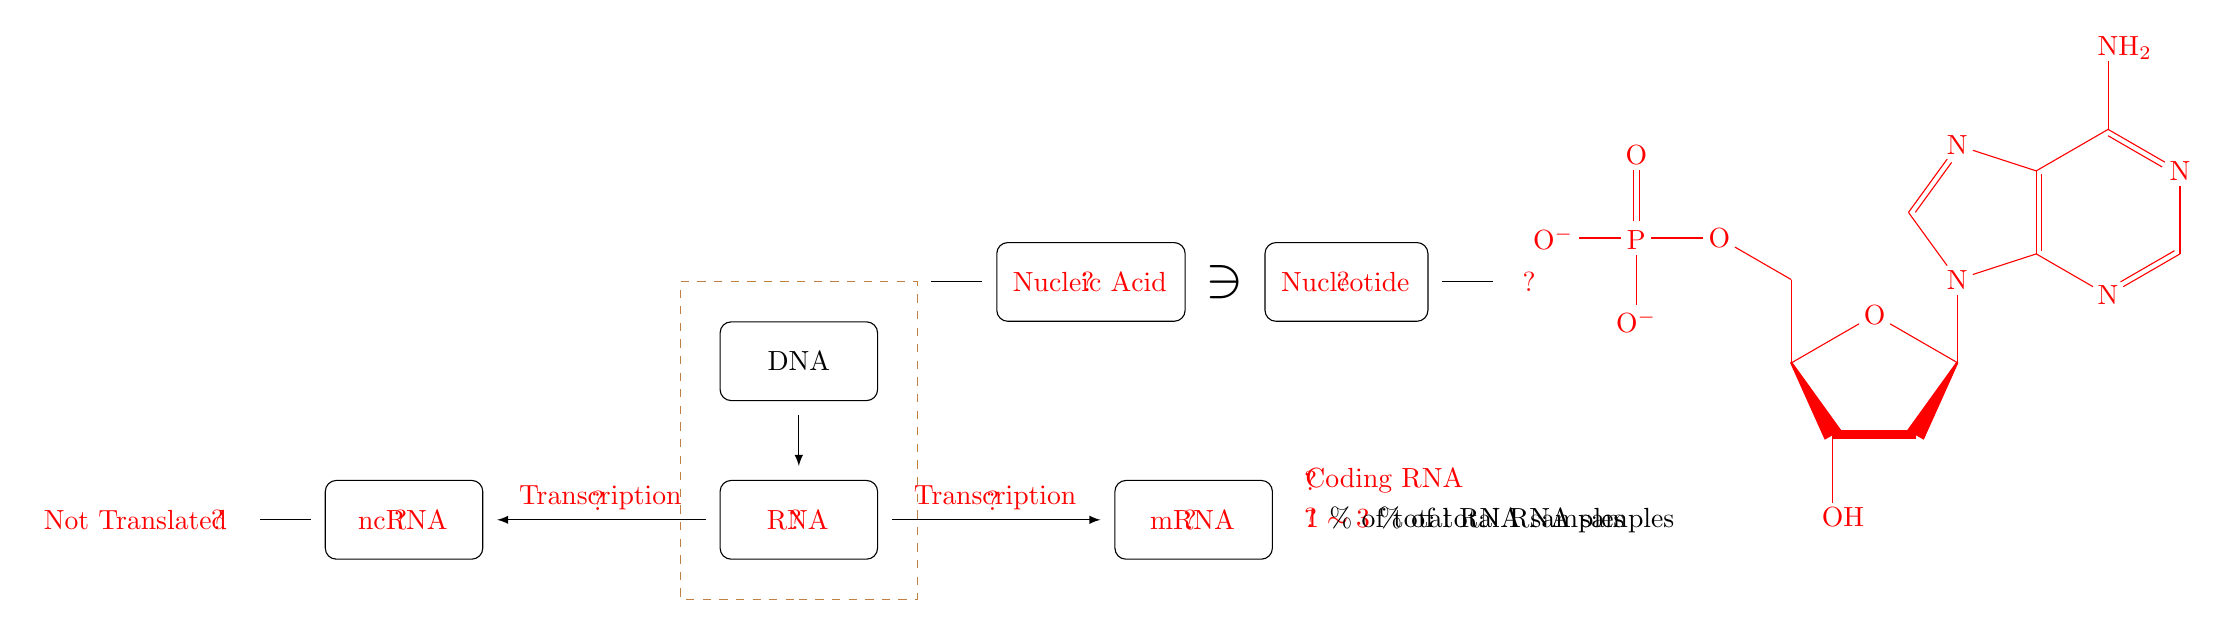
\begin{tikzpicture}
        \node[default, draw](dna){DNA};
\question{below=of dna}{rna}{RNA}{?}
\draw[arrow](dna) to (rna);
\question{right=3cm of rna}{mrna}{mRNA}{?}
\question{left=3cm of rna}{ncRna}{ncRNA}{?}
\draw[arrow](rna) to coordinate(rnaToMrna) (mrna);
\comment{above=0 of rnaToMrna}{transcription}{Transcription}{?}
\draw[arrow](rna) to coordinate(rnaToNcRna) (ncRna);
\comment{above=0 of rnaToNcRna}{ncRnaText}{Transcription}{?}
\comment{right=.2 of mrna}{mrnaText}{$1\sim 3$ \textcolor{black}{\% of total RNA samples}}{? \textcolor{black}{\% of total RNA samples}}
\comment{above=.5 of mrnaText.west, anchor=west}{mrnaTextFirst}{Coding RNA}{?}
\comment{left=of ncRna}{ncRnaTextSecond}{Not Translated}{?}
\draw[line](ncRna) to (ncRnaTextSecond);
\draw[dashed, brown]($(rna.south)+(0,-.5)$)
-| ($(dna.east)+(.5,0)$) |- coordinate(nucleicAcid) ($(dna.north)+(0,.5)$) -| ($(rna.west)+(-.5,0)$) |- cycle;
\question{right=of nucleicAcid}{nucleicAcidText}{Nucleic Acid}{?}
\draw[line](nucleicAcid) to (nucleicAcidText);
\question{right=of nucleicAcidText}{nucleotide}{Nucleotide}{?}
\node at($(nucleicAcidText.east)!.5!(nucleotide.west)$){\huge$\ni$};
\comment{right=of nucleotide}{nucleotideStructure}
{
\chemfig{
O^{-}-P(=[:90]O)(-[:-90]O^{-})-O
-[:-30]-[:-90]([:-18]<[:-60](-[6]OH)-[0,,,,line width=3pt]>[:60]
(-[:90]N
*5([:72]-
*6(-N=-N=(-NH_2)-=)
--N=-))
-[:150,1.15]O-[:210,1.15])
}}{?}
\draw[line](nucleotide) to (nucleotideStructure);

    \end{tikzpicture}
    \chemmove{
        \draw[arrow, blue](hydrogen1) to (oxygen1);
        \commentAt{$(oxygen2)!.5!(hydrogen2)+(-.35,0)$}{fivePrime}{$5^{\prime}$ Carbon}{?}
        \commentAt{$(oxygen3)!.5!(hydrogen3)+(-.1,.1)$}{threePrime}{$3^{\prime}$ Carbon}{?}
        \coordinate(glycosidicBond) at($(nitrogen1)!.5!(hydrogen5)$);
        \comment{above left=2.5 of glycosidicBond}{glycosidicBondText}{Glycosidic Bond}{?}
        \draw[line, dotted](glycosidicBond) to ($(glycosidicBondText.east)+(-.2,0)$);
    }
\end{inctext}
\begin{inctext}[label={overlay}, overlay={\node at($(page.north)+(0,-3)$){\Huge Soma};}]
    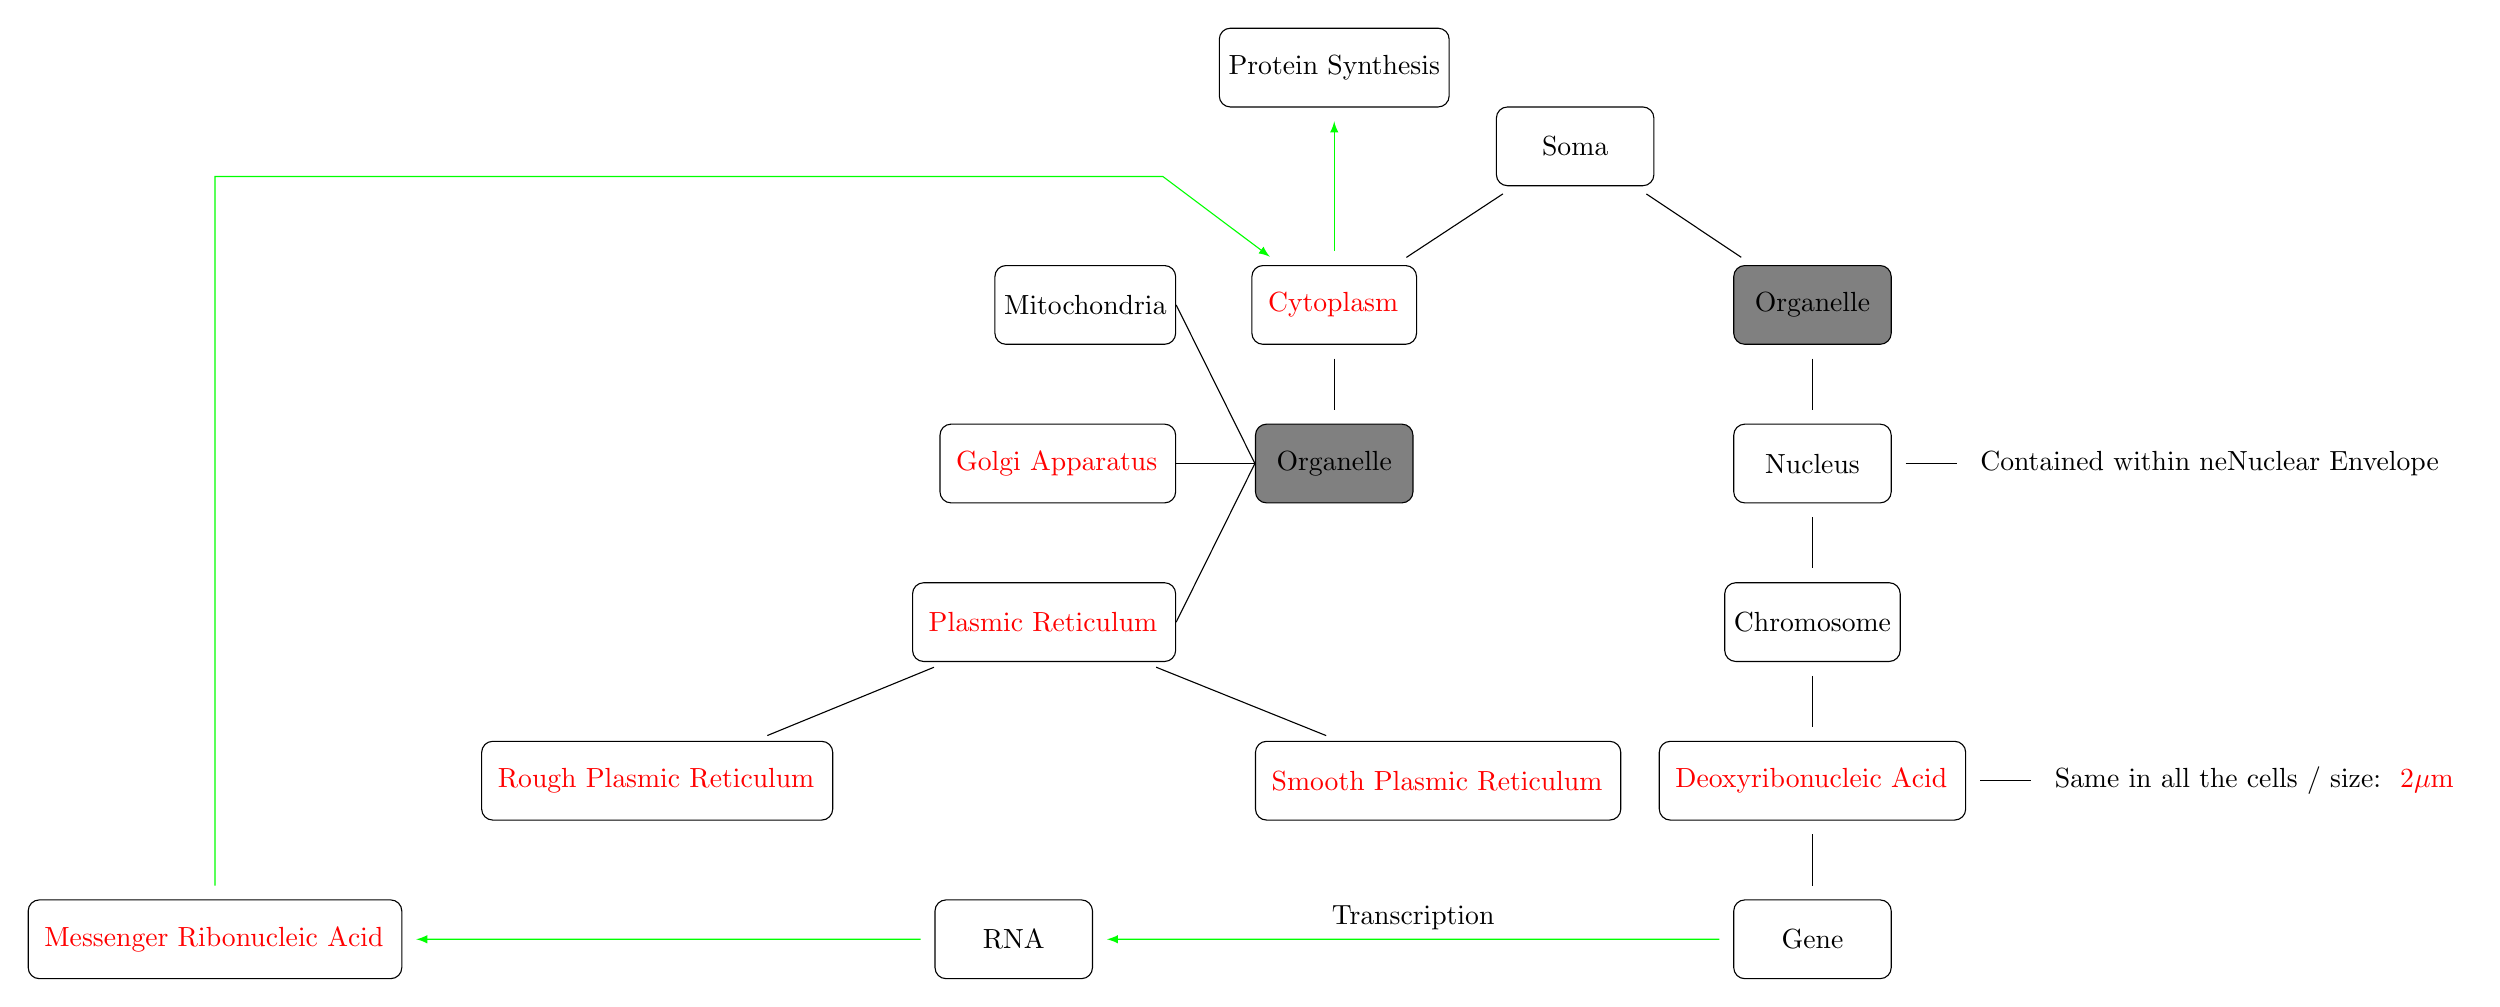
\begin{tikzpicture}
        \node[default, draw](soma){Soma};

\node[default, draw, below left=of soma, switch ocg={cytoplasm}](cytoplasm){
    \basic{cytoplasm}{Cytoplasm}
};
\node[above left=of cytoplasm](space1){};
\node[default, draw, above=2cm of cytoplasm](proteinsynthesis){Protein Synthesis};

\node[default, draw, below right=of soma, fill=gray](organelle2){Organelle};

\node[default, draw, below=of cytoplasm, fill=gray](organelle1){Organelle};
\node[default, draw, below=of organelle2](nucleus){Nucleus};
\node[right=of nucleus, switch ocg={ne}](nuclear envelope){Contained within
    \basicc{ne}{Nuclear Envelope}
};

\node[default, draw, above left=of organelle1](mitochondria){Mitochondria};
\node[default, draw, left=of organelle1, switch ocg={ga}](golgi apparatus){
    \basic{ga}{Golgi Apparatus}
};
\node[default, draw, below left=of organelle1, switch ocg={pr}](plasmic reticulum){
    \basic{pr}{Plasmic Reticulum}
};


\node[default,draw, below left=of plasmic reticulum, switch ocg={rpr}](rough plasmic reticulum){
    \basic{rpr}{Rough Plasmic Reticulum}
};
\node[default, draw, below right=of plasmic reticulum, switch ocg=spr](smooth plasmic reticulum){
    \basic{spr}{Smooth Plasmic Reticulum}
};

\node[default, draw, below=of nucleus](chromosome){Chromosome};
\node[default, draw, below=of chromosome, switch ocg={da}](deoxyribonucleic acid){
    \basic{da}{Deoxyribonucleic Acid}
};
\node[right=of deoxyribonucleic acid, switch ocg={nano}](2nm){
    Same in all the cells / size:\basic{nano}{2$\mu$m}
};
\node[default, draw, below=of deoxyribonucleic acid](gene){Gene};
\node[default, draw, below left=of rough plasmic reticulum, switch ocg={mra}](mrna){
    \basic{mra}{Messenger Ribonucleic Acid}
};
\node[default, draw](rna)at ($(mrna)!.5!(gene)$){RNA};

% ------------------------------------ Arrows -----------------------------------------------------------

\draw[line](soma) to (cytoplasm);
\draw[line](soma) to (organelle2);

\draw[line](organelle2) to (nucleus);

\draw[line](cytoplasm) to (organelle1);

\draw[-](organelle1.west) to (mitochondria.east);
\draw[-](organelle1.west) to (golgi apparatus.east);
\draw[-](organelle1.west) to (plasmic reticulum.east);

\draw[line](plasmic reticulum) to (rough plasmic reticulum);
\draw[line](plasmic reticulum) to (smooth plasmic reticulum);

\draw[line](nucleus) to (chromosome);
\draw[line](nucleus) to (nuclear envelope);

\draw[line](chromosome) to (deoxyribonucleic acid);

\draw[line](deoxyribonucleic acid) to (gene);
\draw[line](deoxyribonucleic acid.east) to (2nm);

\draw[arrow, green](gene) to node[above, black]{Transcription} (rna);
\draw[arrow, green](rna) to (mrna);
\draw[arrow, green](mrna) |- (space1.center) to (cytoplasm);
\draw[arrow, green](cytoplasm) to (proteinsynthesis);
    \end{tikzpicture}
\end{inctext}
\section*{Why a Triplet Code?}
Prior to understanding the details of transcription and translation, geneticists predicted that DNA could encode amino acids only if a code of at least three nucleotides was used. The logic is that the nucleotide code must be able to specify the placement of 20 amino acids. Since there are only four nucleotides, a code of single nucleotides would only represent four amino acids, such that A, C, G and U could be translated to encode amino acids. A doublet code could code for 16 amino acids (4 x 4). \hl{A triplet code could make a genetic code for 64 different combinations (4 X 4 X 4) genetic code and provide plenty of information in the DNA molecule to specify the placement of all 20 amino acids.} When experiments were performed to crack the genetic code it was found to be a code that was triplet. These three letter codes of nucleotides (AUG, AAA, etc.) are called codons.\\
The genetic code only needed to be cracked once because it is universal (with some rare exceptions). That means all organisms use the same codons to specify the placement of each of the 20 amino acids in protein formation. A codon table can therefore be constructed and any coding region of nucleotides read to determine the amino acid sequence of the protein encoded. A look at the genetic code in the codon table below reveals that the code is redundant meaning many of the amino acids can be coded by four or six possible codons. The amino acid sequence of proteins from all types of organisms is usually determined by sequencing the gene that encodes the protein and then reading the genetic code from the DNA sequence.
\\\\src: \url{https://passel2.unl.edu/view/lesson/3ccee8500ac8/6}
\newpage
\section*{tRNA}
While the specific nucleotide sequence of an mRNA specifies which amino acids are incorporated into the protein product of the gene from which the mRNA is transcribed, \hl{the role of tRNA is to specify which sequence from the genetic code corresponds to which amino acid.} The mRNA encodes a protein as a series of contiguous codons, each of which is recognized by a particular tRNA. One end of the tRNA matches the genetic code in a three-nucleotide sequence called the anticodon. The anticodon forms three complementary base pairs with a codon in mRNA during protein biosynthesis.

On the other end of the tRNA is a covalent attachment to the amino acid that corresponds to the anticodon sequence. Each type of tRNA molecule can be attached to only one type of amino acid, so each organism has many types of tRNA. Because the genetic code contains multiple codons that specify the same amino acid, there are several tRNA molecules bearing different anticodons which carry the same amino acid.

The covalent attachment to the tRNA $3^{\prime}$ end is catalysed by enzymes called aminoacyl tRNA synthetases. During protein synthesis, tRNAs with attached amino acids are delivered to the ribosome by proteins called elongation factors, which aid in association of the tRNA with the ribosome, synthesis of the new polypeptide, and translocation (movement) of the ribosome along the mRNA. If the tRNA's anticodon matches the mRNA, another tRNA already bound to the ribosome transfers the growing polypeptide chain from its $3^{\prime}$ end to the amino acid attached to the $3^{\prime}$ end of the newly delivered tRNA, a reaction catalysed by the ribosome. A large number of the individual nucleotides in a tRNA molecule may be chemically modified, often by methylation or deamidation. These unusual bases sometimes affect the tRNA's interaction with ribosomes and sometimes occur in the anticodon to alter base-pairing properties.
\\\\src: \url{https://en.wikipedia.org/wiki/Transfer_RNA}
\end{document}